%%%%%%%%%%%%%%%%%%%%%%%%%%%%%%%%%%%%%%%%%%%%%%%%%%%%%%%%%%%%%%%%%%%%%%%%%%%%%%%%
%%%%%%%%%%%%%%%%%%%%%%%%%%%%%%%%%%%%%%%%%%%%%%%%%%%%%%%%%%%%%%%%%%%%%%%%%%%%%%%%
\exercice{Analyse de la réponse temporelle d'un SLCI~\moyen}
%%%%%%%%%%%%%%%%%%%%%%%%%%%%%%%%%%%%%%%%%%%%%%%%%%%%%%%%%%%%%%%%%%%%%%%%%%%%%%%%
%%%%%%%%%%%%%%%%%%%%%%%%%%%%%%%%%%%%%%%%%%%%%%%%%%%%%%%%%%%%%%%%%%%%%%%%%%%%%%%%
Nous avons relevé la reponse à un échelon unitaire, 
declenchée à $t=0$, d'un système linéaire.
Cette réponse est donnée sur la figure~\ref{fig-2nd} ci-dessous.
L'objectif de cet exercice est de caractériser le système 
à partir de cette réponse temporelle.
%-------------------------------------------------------------------------------
\begin{figure}[!h]
    \centering
    \tikzsetnextfilename{exercice_reponse-2nd_chap-model-ext}
    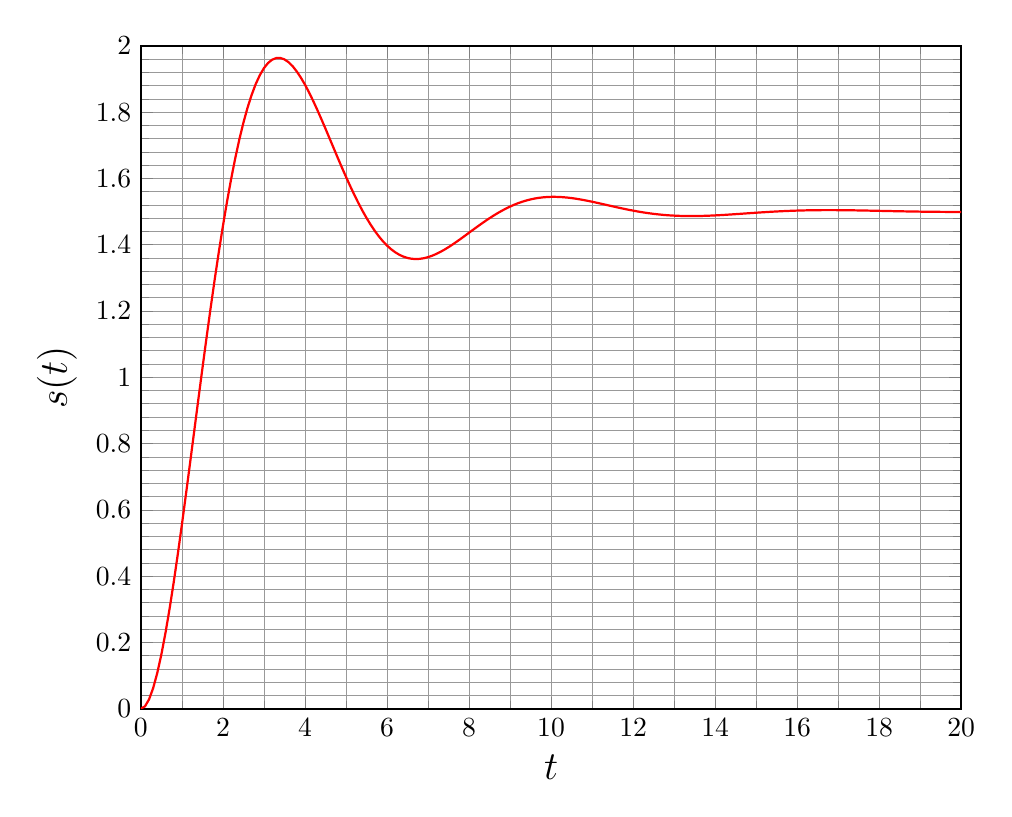
\begin{tikzpicture}
    \pgfmathsetmacro{\kk}{1.5}
    \pgfmathsetmacro{\zz}{0.35}
    \pgfmathsetmacro{\wz}{1.0}
    \pgfmathsetmacro{\aa}{\zz*\wz}
    \pgfmathsetmacro{\bb}{sqrt(1-\zz*\zz)}
    \pgfmathsetmacro{\wwd}{\wz*\bb}
    \pgfmathsetmacro{\mm}{1.0/\bb}
    \pgfmathsetmacro{\pp}{acos(\zz)}
    \begin{axis}[
        width=12cm,
        height=10cm,
        legend style={draw=none},
        legend pos=south west,
        axis line style = thick,
        xmin=0,
        xmax=20,
        ymin=0,
        ymax=2,
        xlabel={$t$},
        ylabel={$s(t)$},
        label style={font=\Large},
        minor y tick num=4,
        minor x tick num=1,
        grid=both,
        grid style={line width=.2pt, draw=gray!80},
        major grid style={line width=.2pt,draw=gray!80},
        ]
    \addplot[thick,color=red,domain=0:20,samples=201]
    {\kk*(1-\mm*exp(-\aa*x)*sin(deg(x)*\wwd+acos(\zz)};%+deg(\pp)))};
    \end{axis}
\end{tikzpicture}


    \caption{Réponse indicielle d'un système linéaire\label{fig-2nd}}
\end{figure}
%-------------------------------------------------------------------------------
%%%%%%%%%%%%%%%%%%%%%%%%%%%%%%%%%%%%%%%%%%%%%%%%%%%%%%%%%%%%%%%%%%%%%%%%%%%%%%%%
\question{Déterminer :}
%%%%%%%%%%%%%%%%%%%%%%%%%%%%%%%%%%%%%%%%%%%%%%%%%%%%%%%%%%%%%%%%%%%%%%%%%%%%%%%%
%-------------------------------------------------------------------------------
\begin{itemize}
    \item l'ordre du système,
    \item le gain statique $K$,
    \item le temps de réponse à 5\%,
    \item et le dépassement relatif en \%.
\end{itemize}
%-------------------------------------------------------------------------------
%%%%%%%%%%%%%%%%%%%%%%%%%%%%%%%%%%%%%%%%%%%%%%%%%%%%%%%%%%%%%%%%%%%%%%%%%%%%%%%%
\question{En déduire l'amortissement $\xi$, la pulsation propre $\omega_0$ et 
écrire la fonction de transfert.}
%%%%%%%%%%%%%%%%%%%%%%%%%%%%%%%%%%%%%%%%%%%%%%%%%%%%%%%%%%%%%%%%%%%%%%%%%%%%%%%%
Nous rappelons que le temps du premier maximum est 
donné par $t_1=\dfrac{\pi}{\omega_d}=\dfrac{\pi}{\omega_0\sqrt{1-\xi^2}}$
et le dépassement par $D=e^{\dfrac{-\xi\pi}{\sqrt{1-\xi^2}}}$
On pourra s'aider des abaques 1 et 2 présentés en annexe.

%%%%%%%%%%%%%%%%%%%%%%%%%%%%%%%%%%%%%%%%%%%%%%%%%%%%%%%%%%%%%%%%%%%%%%%%%%%%%%%%
\question{Calculer les pôles du système et les placer les sur une cartes des
pôles (plan complexe).}
%%%%%%%%%%%%%%%%%%%%%%%%%%%%%%%%%%%%%%%%%%%%%%%%%%%%%%%%%%%%%%%%%%%%%%%%%%%%%%%%
\clearpage
%%%%%%%%%%%%%%%%%%%%%%%%%%%%%%%%%%%%%%%%%%%%%%%%%%%%%%%%%%%%%%%%%%%%%%%%%%%%%%%%
%%%%%%%%%%%%%%%%%%%%%%%%%%%%%%%%%%%%%%%%%%%%%%%%%%%%%%%%%%%%%%%%%%%%%%%%%%%%%%%%
\exercice{Détermination de la fonction de transfert~\facile}
%%%%%%%%%%%%%%%%%%%%%%%%%%%%%%%%%%%%%%%%%%%%%%%%%%%%%%%%%%%%%%%%%%%%%%%%%%%%%%%%
%%%%%%%%%%%%%%%%%%%%%%%%%%%%%%%%%%%%%%%%%%%%%%%%%%%%%%%%%%%%%%%%%%%%%%%%%%%%%%%%
On souhaite déterminer les fonctions de transfert donnant lieu à réponse 
indicielle ayant certaines caractéristiques.
\acpl


